\documentclass[11pt]{article}

\usepackage[margin=1in]{geometry}
\usepackage[T1]{fontenc}
\usepackage[utf8]{inputenc}
\usepackage{lmodern}
\usepackage{microtype}
\usepackage{xcolor}
\usepackage{booktabs}
\usepackage{array}
\usepackage{tabularx}
\usepackage{enumitem}
\usepackage[most]{tcolorbox}
\usepackage{graphicx}
\usepackage{hyperref}
\usepackage{xurl}
\usepackage{fancyhdr}
\usepackage{titlesec}
\usepackage{float}

\definecolor{AccentBlue}{RGB}{37,84,124}
\definecolor{SoftBlue}{RGB}{237,244,250}
\definecolor{SoftGray}{RGB}{248,248,248}

\hypersetup{
  colorlinks=true,
  linkcolor=AccentBlue,
  urlcolor=AccentBlue
}
\urlstyle{same}

\setlength{\parindent}{0pt}
\setlength{\parskip}{0.65em}
\setlist[itemize]{topsep=0.25em,itemsep=0.2em,leftmargin=1.3em}
\setlist[enumerate]{topsep=0.25em,itemsep=0.2em,leftmargin=1.4em}

\titleformat{\section}{\large\bfseries\color{AccentBlue}}{\thesection.}{0.55em}{}
\titleformat{\subsection}{\normalsize\bfseries\color{AccentBlue}}{\thesubsection}{0.5em}{}
\titlespacing*{\section}{0pt}{1.0em}{0.35em}
\titlespacing*{\subsection}{0pt}{0.8em}{0.25em}

\pagestyle{fancy}
\fancyhf{}
\fancyhead[L]{\textcolor{AccentBlue}{David Hardin et al.}}
\fancyhead[R]{\textcolor{AccentBlue}{Enterprise-Grade Copilot SCP Extension}}
\fancyfoot[C]{\thepage}
\setlength{\headheight}{14pt}

\newtcolorbox{summarybox}{
  colback=SoftBlue,
  colframe=AccentBlue,
  boxrule=0.7pt,
  arc=2.5pt,
  left=8pt,right=8pt,top=7pt,bottom=7pt
}

\newcolumntype{Y}{>{\raggedright\arraybackslash}X}

\begin{document}

%\begin{center}
{\LARGE\bfseries\color{AccentBlue} Enterprise-Grade Copilot SCP Extension for INSPECTA\par}
\vspace{0.35em}
{\large David Hardin, Amer Tahat, Isaac Aumndson and Darren Cofer\par}
{\normalsize April 2026\par}
%\end{center}


\section*{Abstract}

This white paper examines whether the current SCP effort can be extended from task-level neuro-symbolic assistance to an enterprise-grade copilot for INSPECTA. We organize the discussion around a threat model that links adversarial content, skill and dependency compromise, policy enforcement, tool execution, and audit paths. The model is used to separate opportunities that are feasible under current funding from commitments that require additional budget, licensing authority, and infrastructure. Four coupled areas are highlighted. First, the orchestrator, skill registry, and feedback loop can be extended from the current Isolette-scale demos toward a firewall-scale demonstration by comparing baseline runs with and without skill files using total, cached, and reasoning tokens, wall-clock time, and verified task completion. Second, any enterprise commitment depends on concrete platform questions about fine-tuning, trajectory fine-tuning, skill-loading mechanisms, agentic workflow access, and token-budget governance. Third, broader deployment expands the attack surface and requires dedicated red-team work on prompt injection, privilege misuse, supply-chain compromise, and denial-of-wallet behavior [13]. Fourth, knowledge transfer across institutions raises additional requirements for isolated hosting, controlled model distribution, and defensible data governance. Under current funding, the first area is actionable; the others should be treated as extension candidates rather than assumed deliverables.


\begin{summarybox}
\textbf{First-page summary.} Recent security literature treats enterprise copilots as automation platforms rather than chat interfaces: once a system can read untrusted content and act through tools, the dominant risks shift to control-flow hijacking, privilege misuse, supply-chain compromise, and data exfiltration. Defense in depth therefore requires least privilege, sandboxed execution, verification gates, provenance for models, prompts, and skills, and end-to-end red teaming rather than prompt-only testing [13].
\end{summarybox}

\begin{figure}[H]
\centering
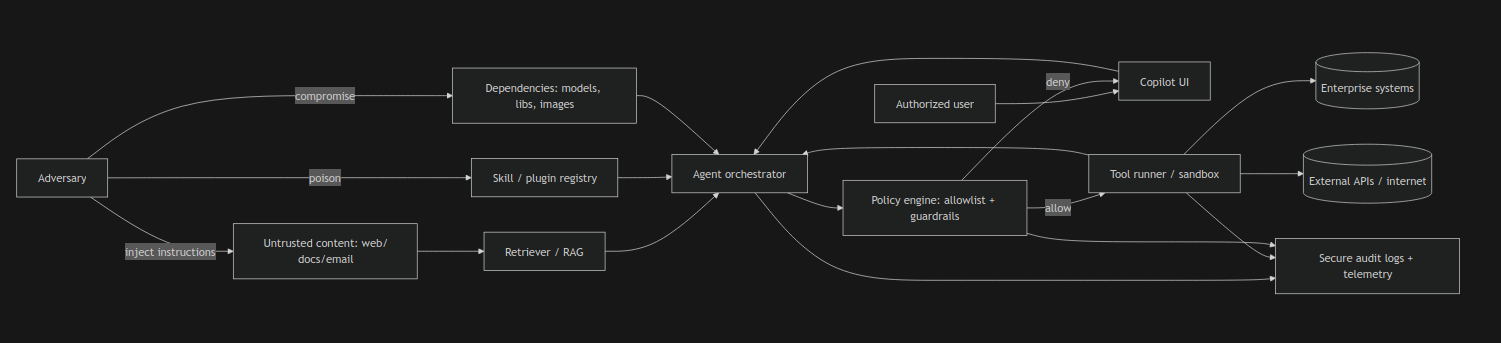
\includegraphics[width=\textwidth]{threat-model.png}
\caption{Threat model for the proposed SCP extension. The model links adversarial content, skill and dependency compromise, the agent orchestrator, the policy engine, tool execution, and audit telemetry. It is the organizing frame for the opportunities and risks discussed in this white paper.}
\label{fig:threat-model}
\end{figure}

\section{Introduction}

The question most relevant to the DARPA discussion is not whether GenAI can simply do the same work faster. The more useful question is what mix of AI assistance, formal tooling, and human review produces the highest verified throughput per unit cost under explicit assumptions. Figure 1 captures that framing as a threat model for the proposed SCP extension. It places the agent orchestrator at the center of a system that must process untrusted inputs, load skill files and dependencies, invoke tools, enforce policy, and preserve auditable behavior. This perspective is useful because it links technical opportunity to budget reality: some parts of the design can be extended now, while others require additional resources and institutional commitments.

The paper therefore organizes the current opportunity around four coupled areas. The first is the orchestrator, skill registry, and feedback loop, which can be extended from the current Isolette-scale work toward a firewall-scale demonstration. The second is enterprise commitment, which depends on platform access, license terms, and tuning authority. The third is red teaming of the copilot itself, because the attack surface grows substantially once the system reads external documents and acts through tools. The fourth is data transferability across organizations, which raises deployment and governance questions that are larger than the present seedling scope.

\section{Area 1: Orchestrator, skill registry, and feedback loop}

The most credible near-term extension is the orchestrator path. In this area, the copilot is asked to consume a document input (for example, a PDF) and generate progressively more formal artifacts and implementation elements with minimal human intervention, while still preserving human validation where required. The key experiment is a controlled baseline-versus-enhanced comparison. The baseline uses the copilot without reusable skill files and without learned feedback structure. The enhanced path uses the same foundation model together with skill files, formal tool calls, and a verifier-mediated feedback loop. This design is a natural fit for the current SCP effort because it can demonstrate value without assuming enterprise deployment.

The evaluation should remain simple and decision-oriented. The decisive metric is not raw model speed, but the amount of verified work completed within a bounded budget.

\begin{table}[H]
\centering
\begin{tabularx}{\textwidth}{>{\bfseries}p{0.30\textwidth}Y}
\toprule
Metric & Use in the baseline-versus-enhanced comparison \\
\midrule
Total tokens & Captures overall inference cost for the task. \\
Cached tokens & Shows how much reusable context and prompt structure are retained across runs. \\
Reasoning tokens & Measures the expensive search component that should decrease as the skill layer matures. \\
Wall-clock time & Captures end-to-end productivity rather than model latency alone. \\
Verified task completion & Records whether the task is completed within budget and accepted by the relevant verifier or reviewer. \\
Human interventions & Measures how often experts must repair, restate, or redirect the workflow. \\
\bottomrule
\end{tabularx}
\caption{Core evaluation metrics for document-to-system demonstrations.}
\label{tab:metrics}
\end{table}

Under current funding, this area is the most actionable. It supports a progression from the existing Isolette-scale demonstrations toward a firewall-scale demonstration, while preserving the central evaluation question: how much verified work can be completed within a fixed token and time budget when the copilot is augmented with reusable skills and formal feedback?

\section{Area 2: Enterprise commitment and platform authority}

A stronger commitment to an enterprise-grade copilot requires answers to platform and licensing questions that materially change the design. At minimum, the team needs to know whether enterprise access permits base-model fine-tuning, trajectory fine-tuning (often described operationally as supervised fine-tuning of selection behavior), explicit skill-file load training, and agentic workflow access beyond a user-facing chatbot surface. The enterprise token budget per user per day, the charging model, and the scope of policy enforcement---enterprise-wide or project-specific---also affect the architecture. If fine-tuning is not available, the near-term design must continue to rely more heavily on supervised Meta-Rules learning, skill files, and external formal tools.

\begin{table}[H]
\centering
\begin{tabularx}{\textwidth}{>{\bfseries}p{0.34\textwidth}Y}
\toprule
Decision question & Why it matters for the design \\
\midrule
Is base-model fine-tuning permitted? & Determines whether adaptation can move from prompt-and-skill control into model weights. \\
Is trajectory fine-tuning available? & Affects whether tool and branch selection can be learned directly rather than scripted indirectly. \\
Can skill-file loading be trained or optimized? & Determines whether reusable workflows remain external artifacts or become part of the adaptation pipeline. \\
Are agentic workflow APIs available? & Distinguishes a true copilot platform from a user-facing chat surface. \\
How are token budgets allocated and charged? & Changes the economics of enterprise-wide versus project-scoped deployment. \\
\bottomrule
\end{tabularx}
\caption{Platform questions that should be answered before making an enterprise commitment.}
\label{tab:enterprise-questions}
\end{table}

\section{Area 3: Red teaming and attack-surface growth}

The third area is the red teaming required when the copilot itself becomes part of the product rather than merely a research aid. Enterprise copilots combine language models with retrieval, memory, tool execution, and skill ecosystems; the result is a security profile closer to an automation platform than a chatbot [1,2,4,6,13]. Once the system can read untrusted documents and act on internal systems, the main risks shift toward instruction injection, privilege misuse, supply-chain compromise, unsafe output handling, and data exfiltration [1,2,7-10]. For that reason, prompt-layer evaluation alone is insufficient. The system requires end-to-end threat modeling, sandboxing, provenance controls, monitoring, and empirical red teaming [13].

This point also explains why naive probabilistic generation is a poor product strategy. Unbounded search trees and repeated retries can amplify both security and cost risk by increasing attack surface, wall-clock time, and token consumption. The more defensible approach is budgeted generation with verifiers, typed tool interfaces, and containment mechanisms such as least privilege, kill switches, and audit trails [2-5,7,8]. Formal methods remain important in this setting, but they complement rather than eliminate the need for continuous adversarial testing.

The attached survey of enterprise-grade copilots emphasizes the same point in broader terms: once language models are connected to retrieval, tool execution, and skill ecosystems, the dominant security problems are no longer limited to unsafe text generation. They include control-flow hijacking, supply-chain compromise, insecure output handling, and operational failure under adversarial load. For that reason, any serious enterprise commitment should budget for both formal assurance where possible and empirical adversarial evaluation where formal coverage is incomplete.

\section{Area 4: Data transferability and isolated deployment}

The fourth area is knowledge and model transferability across institutions. At present, much of that process still depends on human pipelines. Once trained models, adapters, or skill packages must move across companies, however, the risk surface increases. A more defensible long-term direction is an isolation-first deployment model in which training and red teaming occur within a protected research environment, after which vetted model images or artifacts are transferred into partner data centers under controlled policies.

This idea is consistent with emerging Federal interest in secure, shared AI infrastructure for scientific work. For example, the White House Genesis Mission describes a secure integrated platform that combines high-performance computing, AI models, datasets, and external partnerships under explicit security and governance controls [11]. An analogous pattern could support knowledge transferability for SCP extensions: collaborators could access trained models or open materials in a controlled environment, while companies would deploy approved images internally rather than share raw development pipelines. In the INSPECTA context, this would be a substantial change to the current TA3 knowledge-transfer assumptions and should be treated as a separate design and budget question.

\section{Implications for the DARPA discussion}

For the DARPA discussion, the most credible near-term message is therefore disciplined optimism. Current funding can support the orchestrator and skill-registry path, including baseline-versus-enhanced measurements and a stronger document-to-system demonstration. It may also support limited threat modeling and selected security experiments. By contrast, a true enterprise-grade copilot requires additional commitments: licensing clarity, red-team capacity, deployment logistics, and a governance model for transferability. Those items should be framed as extension candidates rather than as obligations of the current budget.

\section{Conclusion}

The proposed SCP extension should be understood as a staged, evaluation-driven program. Near-term work can demonstrate that neuro-symbolic orchestration improves verified throughput by combining skill files, formal tools, and feedback loops around the existing INSPECTA toolchain and further optimized using the supervised self-adaptation Meta-Rules learning algorithm. Longer-term enterprise deployment remains promising, but only if the program explicitly funds the additional work needed for platform commitment, red teaming, and cross-institution transferability.

\begin{thebibliography}{13}

\bibitem{greshake2023}
Johann Greshake et al.
\newblock \emph{Not What You've Signed Up For: Compromising Real-World LLM-Integrated Applications with Indirect Prompt Injection}.
\newblock arXiv:2302.12173, 2023.
\newblock \url{https://arxiv.org/abs/2302.12173}.

\bibitem{owasp2025}
OWASP Foundation.
\newblock \emph{OWASP Top 10 for Large Language Model Applications}.
\newblock OWASP Project.
\newblock \url{https://owasp.org/www-project-top-10-for-large-language-model-applications/}.

\bibitem{nist800207}
Scott Rose et al.
\newblock \emph{Zero Trust Architecture}.
\newblock NIST SP 800-207, National Institute of Standards and Technology, 2020.
\newblock \url{https://csrc.nist.gov/pubs/sp/800/207/final}.

\bibitem{nistai100}
National Institute of Standards and Technology.
\newblock \emph{Adversarial Machine Learning: A Taxonomy and Terminology of Attacks and Mitigations}.
\newblock NIST AI 100-2e2025.
\newblock \url{https://nvlpubs.nist.gov/nistpubs/ai/NIST.AI.100-2e2025.pdf}.

\bibitem{nistai600}
National Institute of Standards and Technology.
\newblock \emph{Artificial Intelligence Risk Management Framework: Generative AI Profile}.
\newblock NIST AI 600-1.
\newblock \url{https://nvlpubs.nist.gov/nistpubs/ai/NIST.AI.600-1.pdf}.

\bibitem{atlas}
MITRE.
\newblock \emph{ATLAS: Adversarial Threat Landscape for Artificial-Intelligence Systems}.
\newblock \url{https://atlas.mitre.org/}.

\bibitem{microsoft2025}
Microsoft.
\newblock \emph{Planning Red Teaming for Large Language Models (LLMs) and Their Applications}.
\newblock Microsoft Learn.
\newblock \url{https://learn.microsoft.com/en-us/azure/foundry/openai/concepts/red-teaming}.

\bibitem{anthropic2025}
Anthropic.
\newblock \emph{Mitigating the Risk of Prompt Injections in Browser Use}.
\newblock Anthropic News.
\newblock \url{https://www.anthropic.com/news/prompt-injection-defenses}.

\bibitem{checkpoint2026}
Check Point Research.
\newblock \emph{ChatGPT Data Leakage via a Hidden Outbound Channel in the Code Execution Runtime}.
\newblock 2026.
\newblock \url{https://research.checkpoint.com/2026/chatgpt-data-leakage-via-a-hidden-outbound-channel-in-the-code-execution-runtime/}.

\bibitem{openai2024}
OpenAI.
\newblock \emph{Diverse and Effective Red Teaming with Auto-Generated Attacks}.
\newblock Technical report.
\newblock \url{https://cdn.openai.com/papers/diverse-and-effective-red-teaming.pdf}.

\bibitem{whitehouse2025}
The White House.
\newblock \emph{Launching the Genesis Mission}.
\newblock Executive Order, November 24, 2025.
\newblock \url{https://www.whitehouse.gov/presidential-actions/2025/11/launching-the-genesis-mission/}.

\bibitem{privilege2026}
\emph{Evaluating Privilege Usage of Agents on Real-World Tools}.
\newblock arXiv:2603.28166, 2026.
\newblock \url{https://arxiv.org/pdf/2603.28166}.

\bibitem{ferrag2026protocol}
Mohamed Amine Ferrag, Norbert Tihanyi, Djallel Hamouda, Leandros Maglaras, Abderrahmane Lakas, and Merouane Debbah.
\newblock \emph{From Prompt Injections to Protocol Exploits: Threats in LLM-Powered AI Agents Workflows}.
\newblock ICT Express 12(2026):353--383, 2026.
\newblock \url{https://doi.org/10.1016/j.icte.2025.12.001}.

\end{thebibliography}

\end{document}
